\section{Data and Measurement Design}
\label{sec:methods}

This section explains how we turn distributed public traces into auditable record-level measures. Figure~\ref{fig:pipeline} summarizes the pipeline. The study starts from two public evidence sources---model-hub repository records and scholarly paper records---and converts visible traces into typed fields for artifact identity, scholarly linkage, provenance, release packages, and integrated curation readiness. Three principles guide the measurement. First, the source of each trace is preserved, because a model-card field, a paper-side link, and a family mention support different claims. Second, denominators are kept separate, because repository records, paper records, and record-supported artifact claims are not interchangeable. Third, judgment-sensitive fields are calibrated through expert audits and sensitivity checks, so strict metadata claims can be separated from broader discovery or collection-organization signals.

\begin{figure*}[!tbp]
    \centering
    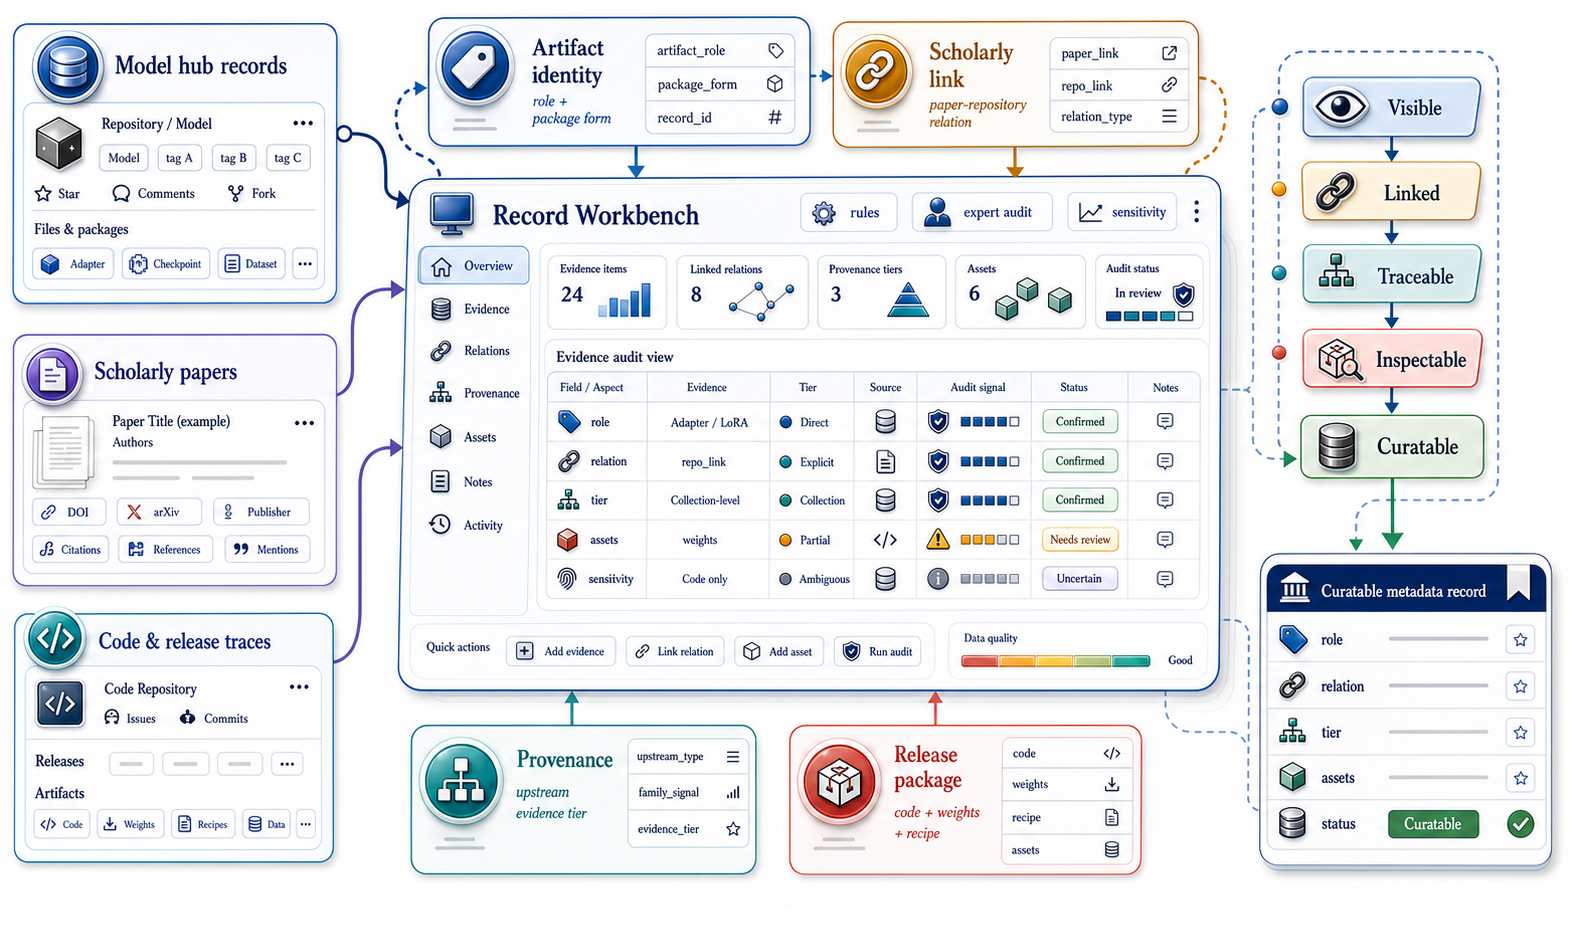
\includegraphics[width=\textwidth]{figures/fig1_overview_gpt_image2_icon_polished_library_crop.png}
    \caption{Overview of the visibility-to-curatability measurement design. Public model-hub, paper, code, and release traces are converted into four typed evidence fields: artifact identity, scholarly linkage, provenance, and release package. Normalization, expert audits, and sensitivity checks distinguish strict evidence, collection-level evidence, and weak or missing evidence before assigning an integrated curation-readiness status.}
    \Description{A workflow diagram with four panels: public traces, evidence extraction, normalization and audit, and curatability decision.}
    \label{fig:pipeline}
\end{figure*}

\begin{table*}[!tbp]
\centering
\caption{Measurement constructs and checks. Each row maps one curation construct to its denominator, signal, calibration check, and supported claim.}
\label{tab:measurement-constructs}
\small
\setlength{\tabcolsep}{3.6pt}
\renewcommand{\arraystretch}{1.08}
\begin{tabular}{@{}p{0.17\linewidth}p{0.18\linewidth}p{0.22\linewidth}p{0.17\linewidth}p{0.18\linewidth}@{}}
\toprule
\textbf{Construct} & \textbf{Unit} & \textbf{Signal} & \textbf{Check} & \textbf{Output claim} \\
\midrule
Artifact identity & 191,375 repos & Role + package form & 300-role audit & Typed identity \\
Scholarly linkage & Repos + 2,214 papers & HF/GitHub links; backlinks & Alignment split & Typed relation \\
Provenance & 2,214 papers & Upstream tier $P$ & 200-row audit & Upstream claim \\
Release package & 2,214 papers & Release tier $R$ & 50-URL audit & Visible assets \\
\textbf{Integrated} & 2,214 papers & \textbf{P/R/L rule} & Sensitivity & \textbf{Readiness status} \\
\bottomrule
\end{tabular}
\renewcommand{\arraystretch}{1.0}
\end{table*}


\subsection{Corpus Construction and Scope}

We built the dataset in four steps: repository collection, paper collection, evidence coding, and validation. The repository collection is a scoped May 2026 query-based snapshot of 191,375 public \hf model repositories. It is designed to capture public records likely to describe compact or derived open \llm artifacts, rather than to serve as a census of all \hf repositories. Query terms were grouped into five buckets---size or compactness, deployment format, derivation or tuning, domain/language/task, and model-family names. Query-bucket sensitivity analysis reports how this scoping affects repository-side measurements.

The repository snapshot contains repository identifiers, owners, creation timestamps, tags, model-family labels, upstream model fields, arXiv references, task descriptors, domain descriptors, and project-inferred artifact role and package-form fields. We treat artifact role and package form as audited inference fields derived from repository metadata and tags. The role taxonomy includes base, fine-tune, adapter/LoRA, merge/mixed, and quantized/deployment records. Package form captures distribution signals such as adapter-only, quantized, converted, checkpoint-complete, code-only, or multi-asset release packaging.

The scholarly corpus combines records from OpenAlex, arXiv metadata, and venue-derived paper lists. After merging and deduplication, it contains 2,729 paper records, corresponding to 2,722 works. We filter these records into a main analysis set of 2,214 paper records, corresponding to 2,208 works, that centrally study compact or derived open \llm artifacts. A paper enters the analysis set when it introduces, adapts, compresses, quantizes, distills, fine-tunes, evaluates, or deploys a compact or derived model artifact as a central research object. Application-only pipelines, general benchmarks, and papers that merely use \llms as tools are excluded unless the compact or derived artifact is itself the object of study.

This scope is operational rather than parameter-count based. ``Compact'' includes strict small models and deployment-oriented compact models. ``Derived'' includes compressed, quantized, distilled, PEFT/adapted, merged, domain-specialized, and evaluation- or deployment-oriented artifacts whose interpretation depends on upstream models or released assets. The anonymized supplementary package lists the query buckets, input sources, construction rules, and derived files used for the reported figures and tables.

\subsection{Evidence Fields and Units of Analysis}

The study uses three denominators. Repository-level percentages describe records in the fixed \hf snapshot. Paper-level percentages describe the 2,214 analysis-set paper records. Artifact-level language refers to curation claims supported by those public records, not to a census of unique model artifacts. This separation is necessary because a paper may discuss multiple model objects, a repository may package an artifact derived from another repository, and the same family name may appear as a target model, parent, teacher, baseline, evaluator, or background context.

Each evidence field supports a distinct curation claim. For scholarly linkage, we keep paper-side \hf links, paper-side GitHub or code-hosting links, repository-side arXiv references, exact model mentions, model-card references, and low-confidence family/size matches as separate signals. These signals differ in evidentiary strength: a paper-side link, a repository backlink, and a matched model mention do not support the same bibliographic claim. In the integrated rubric, the linkage component $L\geq1$ is triggered by one direct alignment signal: an exact \hf edge, an explicit paper-side \hf link, or an explicit paper-side GitHub/code-hosting link. Low-confidence fuzzy matches are retained for sensitivity analysis but do not by themselves satisfy this direct-linkage threshold.

For provenance, we assign each analysis-set paper record to the strongest upstream-evidence tier supported by public records. Stronger tiers require explicit or canonical upstream evidence, such as a visible upstream-model field, a paper statement that the artifact is based on a named checkpoint, or a matched repository whose upstream relation is visible. Lower tiers capture curated-inventory family support, weak contextual family clues, or no usable signal. A paper-repository link may help locate the relevant record, but it supports provenance only when the linked record or paper text exposes an upstream relation. This tiering measures public-record sufficiency, not complete model genealogy.

For release packages, we use a five-level hierarchy: no explicit release signal; stated or incomplete release signal; code, scripts, or recipe; checkpoint, adapter, data, or evaluation asset; and multiple assets or a full recipe. The hierarchy treats openness as visible record evidence for curation. It does not claim that released assets execute successfully or reproduce the reported results.

Table~\ref{tab:measurement-constructs} summarizes the relationship among constructs, denominators, evidence sources, calibration checks, and curation claims. The design keeps visible traces typed: a model-card field, a paper-side link, a family mention, and a release statement are not interchangeable records. They become useful for digital-library curation when their source, calibration evidence, and supported use are retained together.

\subsection{Coding, Calibration, and Audits}

The dataset combines structured Web records with unstructured scholarly text, so we separate three classes of fields. Native fields, such as repository identifiers, timestamps, tags, upstream-model fields, arXiv references, paper metadata, and URLs, are treated as observed public metadata. Rule-derived fields, such as query buckets, denominators, alignment tiers, release-evidence levels, and curatability scores, are generated by deterministic scripts from documented inputs. Judgment-sensitive fields, such as paper inclusion, artifact role, provenance sufficiency, and release-evidence interpretation, are calibrated through expert audits or agreement checks.

LLM-assisted coding is used only as an evidence-extraction aid for paper text. The prompts return structured candidate fields and short supporting excerpts from extracted paper sections. No reported aggregate label is taken directly from a generative output. Final analytical fields are produced after schema validation, rule-based normalization, curated-inventory matching, link-table resolution, and expert-calibrated decision boundaries. The prompt template, extraction schema, model settings, raw candidate outputs, and detailed agreement statistics are documented in the supplementary reproducibility files. The main JCDL measures are artifact role, scholarly linkage, provenance sufficiency, release-package evidence, and integrated curatability.

We report three construct-specific audit layers in the main text. A balanced repository-role audit reviews 300 repositories, with 60 predicted records per role, and checks whether public metadata supports the assigned primary role or suggests a role change or package-form ambiguity. A targeted upstream-evidence audit reviews 200 paper-level provenance rows and distinguishes strict unique-primary support from usable family-level support. A release audit reviews 50 URL or asset-signal rows and checks whether extracted release categories match visible public evidence. These samples calibrate boundary interpretation rather than estimate corpus-wide prevalence; aggregate labels remain rule-based and reproducible. We also report query-bucket sensitivity, alignment-signal decomposition, and curatability-threshold sensitivity.

\begin{table*}[!tbp]
\centering
\caption{Expert-audit outcomes with Wilson 95\% intervals. Audits calibrate boundary decisions rather than estimate population prevalence.}
\label{tab:audit-wilson-ci}
\small
\setlength{\tabcolsep}{5pt}
\renewcommand{\arraystretch}{1.14}
\begin{tabularx}{0.94\textwidth}{@{}p{0.16\textwidth}p{0.21\textwidth}cp{0.18\textwidth}Y@{}}
\toprule
\textbf{Audit layer} & \textbf{Boundary checked} & \textbf{Count} & \textbf{Estimate (95\% CI)} & \textbf{Audit implication} \\
\midrule
Repository role & Strict role support & 256/300 & \cellcolor{TableGreen}\textbf{85.3\%} [80.9, 88.9] & Artifact-role labels are stable \\
\midrule
Upstream evidence & Strict unique-primary & 56/200 & \cellcolor{TableRed}28.0\% [22.2, 34.6] & Strict lineage claims stay conservative \\
 & Usable family-level & 158/200 & \cellcolor{TableGreen}\textbf{79.0\%} [72.8, 84.1] & Family-level grouping is usable \\
\midrule
Release evidence & URL/asset category retained & 50/50 & \cellcolor{TableGreen}\textbf{100.0\%} [92.9, 100.0] & Release categories are stable \\
\bottomrule
\end{tabularx}
\renewcommand{\arraystretch}{1.0}
\end{table*}


\subsection{Integrated Curatability Rubric}

We synthesize provenance, release, and linkage evidence into an integrated curatability rubric. The rubric does not rank model quality, adoption, or executable reproducibility. Each threshold corresponds to a distinct curator task: discovery, grouped inspection, bibliographic control, provenance-aware preservation triage, or multi-asset review.

The provenance component ranges from 0 to 3: no usable provenance, weak contextual clue, curated-inventory family support, and exact or canonical upstream signal. The release component ranges from 0 to 4 using the hierarchy above. The linkage component ranges from 0 to 2: no direct signal, one direct linkage signal, and two or more signals. A \textit{discovery-ready} record contains at least one useful provenance, release, or link signal. The \textit{operational P+R} threshold requires usable provenance and code/recipe-or-stronger release evidence. The \textit{operational+link} sensitivity adds at least one direct linkage signal. The \textit{high-curatability} threshold requires usable provenance, asset-level release evidence, and at least one direct linkage signal. The \textit{preservation-review candidate} threshold further requires a multi-asset or full-recipe release package.

For example, a paper record with an explicit \hf link, a visible upstream base-model relation, and released adapter weights receives link evidence, usable provenance evidence, and asset-level release evidence; it satisfies the high-curatability threshold. A paper record with only a family name and a statement that resources will be released remains useful for discovery, but falls below the operational P+R threshold because the release package is not concrete.

The threshold ladder maps each numerical rule to a curator task. Provenance score $P\geq2$ supports at least family-level collection organization or attribution triage. Release score $R\geq2$ means that code, scripts, or recipe evidence is visible for inspection. Release score $R\geq3$ adds an asset-level package such as a checkpoint, adapter, data, or evaluation asset. Linkage score $L\geq1$ supports bibliographic control through a direct alignment signal. The strictest rule, $P\geq2$, $R\geq4$, and $L\geq1$, identifies preservation-review candidates with multi-asset packages; it is still not an execution test.

The operational+link sensitivity changes the count only marginally because almost all records satisfying $P\geq2$ and $R\geq2$ also contain at least one direct alignment signal under the broad $L$ definition. This is why the main bottleneck is not link evidence after provenance and concrete release evidence are already present, but the co-occurrence of usable provenance and concrete release evidence in the first place.
